\chapter{Теоретическое введение}

\section{Гедонические игры}
Введем определение гедонической игры, которое будет использоваться на протяжении всего исследования.\\

Пусть есть множество агентов $\{1,...,N\}$, $\sigma$ - некоторое разбиение агентов на сообщества, $\sigma=\{S_1,...,S_n,\textbf{ }S_i\cap S_j=\emptyset,\textbf{ }\cup_i S_i=\{1,...,N\}\}$. Агентов будем также называть игроками. Для каждого агента задана функция полезности $u_i(\sigma)$ (или, иначе, функция прибыли), зависящая от текущего разбиения. Пусть агенты могут свободно перемещаться между кластерами. В данной работе \textit{стратегией} игрока будем называть сообщество, которое данный игрок выбирает. Задача состоит в том, чтобы отыскать \textit{оптимальные стратегии} для каждого игрока: то есть, при выборе данной стратегии игрок имеет максимальную прибыль при фиксированных оптимальных стратегиях всех остальных игроков. В данной работе мы будем рассматривать \textit{некооперативные} игры. Это означает, что два или более игрока не могут действовать согласованно, то есть каждый игрок выбирает стратегию, принимая во внимание только собственную прибыль (\textit{"selfish"} players). Результирующее разбиение, в котором никакой игрок не хочет изменить стратегию, и будет искомым разбиением множества агентов на сообщества.\\

Будем называть игру \textit{гедонической}, если функция полезности $u_i$ каждого игрока зависит только от того, какие еще игроки входят в сообщество, которому принадлежит рассматриваемый игрок. При этом разбиение оставшихся вершин на сообщества никак не влияет на прибыль рассматриваемого игрока. С помощью некооперативных гедонических игр можно моделировать множество ситуаций, в которых агенты объединяются в сообщества, исходя из личных интересов. Впервые гедонические игры были введены и проанализированы в этой работе \cite{firsthg}. Большинство работ по гедоническим играм посвящено изучению \textit{равновесия Нэша} (набора оптимальных стратегий игроков, при которых никакой игрок не хочет изменить свою стратегию при фиксированных оптимальных стратегиях других игроков), а также нахождению оптимальных стратегий игроков, доказательству существования или отсутствия равновесия Нэша в различных игровых моделях \cite{core1}, \cite{core2}, \cite{core3}.\\

Чтобы лучше понять, как могут быть устроены гедонические алгоритмы поиска сообществ, рассмотрим примеры конкретных алгоритмов и решаемых ими задач. Как и в метрических алгоритмах кластеризации, количество кластеров в некоторых теоретико-игровых алгоритмах известно заранее, а в других - нет. Приведем несколько существующих алгоритмов.\\

Кластеризацию первого типа в литературе часто называют "fixed clustering". Примедем пример такого алгоритма, кластеризующего полный взвешенный неориентированный граф. Назовем условно веса ребер графа "расстояниями". Пусть число кластеров известно заранее и равно $k$. В таком случае удобно формировать кластеры вокруг так называемых "центроидов" - представителей каждого из $k$ кластеров. Введем "цену" кластера - сумму расстояний от всех агентов в данном кластере до его центроида. Тогда введем цену $c_v(C)$, которую платит агент $v$ за нахождение в кластере $C$, как цену кластера $C$, разделенную поровну между его агентами. Теперь прибыль игрока можно считать равной $-c_v$. Набор стратегий игрока - $k$ чисел, обозначающих номера кластеров, которые можно выбрать. На каждом шаге игроку $v$ нужно выбрать такой кластер $C$, что величина $c_v(C\cup v)$ минимальна, где $c_v$ - "цена", которую платит $v$ при заданном разбиении на сообщества. Оказывается, что агенту нужно минимизировать собственное расстояние до центроида \cite{clusteringhg}. Примером применения такого алгоритма является организация передачи данных между устройствами, минимизирующая энергетические затраты: устройства объединяются в кластеры согласно приведенному алгоритму, и передача данных осуществляется только между агентом и центроидом одного кластера и между центроидами.\\

Кластеризация второго типа имеет еще более широкое применение, так как зачастую количество кластеров заранее неизвестно. Пусть известны только "отношения" между агентами - веса ребер графа. Предположим, что между агентами теперь задана метрика: $d:(, v)\rightarrow [0,1]$. Пусть $d(u, v)$ обозначает "меру различия" объектов $u$ и $v$: если $d(u, v)$ близко к нулю, то объекты похожи, а если, напротив, $d(u, v)$ близко к единице, то объекты очень разные. Пусть также каждый агент $v$ имеет вес $w_v$, обозначающий "меру влияния" на остальных. Пусть агенты хотят быть в одном кластере с близкими им объектами с большим весом, но отделиться непохожих на них агентов с маленьким весом. С помощью функции полезности агента можно это учесть \cite{clusteringhg}. Так можно решать любую задачу, в которой, например, агенты хотят объединиться "по интересам", отдалившись от тех, кто на них не похож.\\

Второй пример важен для нас в данной работе, так как мы будем рассматривать именно этот тип кластеризации, когда количество кластеров заранее неизвестно. Кроме того, мы будем использовать похожую функцию полезности, но функция веса ребер графа $d(u, v)$ уже не будет метрикой, и даже не будет определена для всех пар вершин. Соответственно, $d(u, v)$ уже нельзя считать расстоянием. Веса вершин в нашей работе также будут использоваться, но будет рассмотрено большое их количество, и зависеть они будут от топологии графа, чего в рассмотренной выше постановке быть не может. Про веса вершин будет подробно рассказано в следующей части теоретического введения. 

\section{Центральности}

Понимание роли каждого элемента системы является важным шагом в изучении поведения этой системы. Мы будем рассматривать кластеризацию ориентированных графов (или, иначе, \textit{сети}) с различной топологией, а значит, разные вершины в такой сети будут иметь разное положение относительно всех остальных. Если рассматривать ребро графа как некоторую характеристику "влияния" одной вершины на другую, то такие характеристики, как количество out-соседей, веса out-ребер, а также то, каким "влиянием" обладают сами out-соседи вершины, может характеризовать "важность" вершины в сети. Такая мера "важности" вершины графа называется \textit{мерой центральности}. Мер центральности можно ввести очень много. Рассмотрим здесь те, которые будем использовать для определения важности вершин в данной работе. Приведенные меры центральности определены для ориентированных графов.

\subsection{Betweenness \cite{betweenness}}
Эта мера широко используется в социальных сетях. Она основана на предположении о том, что, если человек в некоторой социальной группе имеет некоторое "центральное" положение, соединяя много пар других людей, то он "важен" для этой группы. Этот человек может в какой-то мере контролировать общение людей, связанных между собой через него кратчайшин путем. В терминах сети, если вершина лежит на большом количестве кратчайших путей между другими вершинами, то мера центральности этой вершины должна быть высокой. Рассмотрим вершины графа $i$ и $j$. Пусть число всех кратчайших путей (называемых также \textit{геодезическими}) из $i$ в $j$ равно $g_{ij}$. Тогда вероятность, что $i$ выберет один из этих путей $p$ для передачи информации $j$, есть $g_{ij}^{-1}$. Тогда для каждой вершины $k$ графа обозначим как $g_{ij}(k)$ число кратчайших путей из $i$ в $j$, содержащих $k$. Тогда мера центральности $k$ вводится следующим образом:
	\begin{equation}
	b_{ij}(k) = \frac{g_{ij}(k)}{g_{ij}},
	\end{equation}
	\begin{equation}
	C_B(k) = \sum_{i<j}b_{ij}(k),
	\end{equation}
	где $b_{ij}(k)$ - вероятость того, что на выбранном пути передачи информации из $i$ в $j$ содержится $k$. 
	
\subsection{Degree}
В некоторых сетях удобно ввести меру центральности так, чтобы она зависела от степени вершины. Например, рассмотрим распространение инноваций в социальных сетях. Чем больше степень вершины, тем больше вершин могут "заразиться" от данной (принять инновацию). В нашей задаче граф ориентированный, поэтому мера центральности вершины будет пропорциональна числу исходящих ребер (out-степени вершины). Обозначим через $d_{max}$ максимальную out-степень вершины в графе. Тогда меру центральности вершины $i$ будем считать так:
	\begin{equation}
	C_d(i) = \frac{\sum_{j\neq i} \delta_{ij}}{d_{max}},
	\end{equation}
	\begin{equation}
	d_{max} = \max_i\{\sum_{j\neq i}\delta_{ij}\},
	\end{equation}
	где $\delta_{ij}=0$, если ребра $i\rightarrow j$ нет, $\delta_ij=1$, если ребро $i \rightarrow j$ есть.\\
	
	Также рассмотрим \textit{weighted} (взвешенную) degree-центральность, в которой важность вершины будет зависеть не только от числа исходящих ребер, но и от их веса (например, в уже рассмотренной социальной сети наличие связи не говорит о том, что информация точно будет передана; вместо этого, можно задать вес ребра как некоторую величину, оценивающую вероятность передачи информации по ребру). Теперь нам потребуется максимальная по всем вершинам сумма весов исходящих ребер в графе: $w_{max}$. Мера центральности вершины $i$:
	\begin{equation}
	C_{wd}(i) = \frac{\sum_{j\neq i} \delta_{ij}\cdot w_{ij}}{w_{max}},
	\end{equation}
	\begin{equation}
	w_{max} = \max_i\{\sum_{j\neq i}\delta_{ij}\cdot w_{ij}\},
	\end{equation}
	где $w_{ij}$ - вес ребра $i \rightarrow j$.
	
	\subsection{Closeness}
	Эта мера центральности, как нетрудно понять из названия, характеризует "близость" вершины ко всем остальным вершинам графа. Пусть $d_{ij}$ - число ребер в кратчайшем пути от вершины $i$ до вершины $j$. Тогда рассмотрим меру:
	\begin{equation}
	D_c(i)=\sum_{j\neq i} d_{ij}.
	\end{equation}
	Указанная величина имеет противоположный смысл: чем меньше сумма кратчайших расстояний от данной вершины до всех остальных, тем более она "центральна". Значит, меру центральности вершины $i$ можно ввести как величину, обратную $D_c(i)$:
	\begin{equation}
	C_c(i) = \frac{1}{\sum_{j\neq i} d_{ij}}.
	\end{equation}
	В уже рассмотренной задаче распространения инноваций closeness-центральность может характеризовать скорость распространения инновации по сети от заданного узла.
	
	\subsection{PageRank \cite{pagerankcent}}
	Центральность вершины в ориентированном графе можно измерить с помощью известного алгоритма ранжирования страниц, соответствующих некоторому поисковому запросу. Согласно алгоритму PageRank, вес страницы А тем больше, чем больше вес страниц В, на нее ссылающихся. Также чем больше страниц В ссылаются на данную страницу А, тем больше вес страницы А. Формулу задают так:
	\begin{equation}
	PR(A)=(1-d)+d\cdot (\frac{PR(T_1)}{C(T_1)}+\dots+\frac{PR(T_n)}{C(T_n)}),
	\end{equation}
	где $PR(A)$ - вычисляемый вес страницы А, $d$ - коэффициент "затухания" (необходим для того, чтобы циклы, появляющиеся, например, если А ссылается на В и В ссылается на А, не "стягивали" на себя всю центральность), $PR(T_i)$ - вес страницы $T_i$, ссылающейся на А, $C(T_i)$ - число ссылок на странице $T_i$, $n$ - число страниц $T_i$, ссылающихся на А \cite{pagerank}.
	
	\subsection{Статические веса}
	Для теоретического исследования алгоритма понадобятся статические веса вершин, которые в работе будут иногда обозначаться \textit{static}. Это означает, что веса всех вершин одинаковы и равны $\frac{1}{2}$.
	
	\subsection{Случайные веса}
	Важности вершин в реальных задачах не всегда зависят от топологии графа: они могут быть получены, например, на основании экспертного мнения. Однако, кластериация такого графа все еще будет зависеть от топологии. Для изучения такого случая можно присвоить вершинам случайные (\textit{random}) веса, лежащие на отрезке $[0,1]$.

\section{Модулярность}
\textit{Модулярностью} будем называть меру качества кластеризации графа. В алгоритмах, использующих модулярность, ищется максимизирующее модулярность разбиение вершин графа на кластеры \cite{modularity}. Модулярность определяется по-разному для ориентированных и неориентированных графов.\\

Мы будем сравнивать результаты работы нашего алгоритма на неориентированном графе с алгоритмами, максимизирующими модулярность, чтобы попробовать понять свойства нашего алгоритма. Поэтому введем вначале определение модулярности для неориентированного графа. Пусть задан неориентированный граф $G=(V,E)$, $|V|=N$, $|E|=m$. Пусть фиксировано разбиение вершин $\sigma=\{S_1,...,S_n,\textbf{ }S_i\cap S_j=\emptyset,\textbf{ }\cup_i S_i=\{1,...,N\}\}$. Модулярность оценивает вероятность существования ребра между двумя вершинами в в неориентированном графе в сравнении с вероятностью его появления в случайной графической модели с тем же распределением по степеням вершин. Например, если ребро оказывается между двумя вершинами с большой степенью, то это неудивительно, и такое ребро вносит небольшой вклад в модулярность. Если же ребро появляется между вершинами с небольшой степенью, то это маловероятное событие, а значит, оно вносит в модулярность больший вклад. Модулярность $q(\sigma)$ разбиения $\sigma$ можно ввести следующим образом:
\begin{equation}
q(\sigma)=\sum_{i=1,\dots,n} [\frac{|E(S_i)|}{m}-(\frac{\sum_{v\in S_i} deg(v)}{2m})^2],
\end{equation}
где $|E(S_i)|$ - число ребер в подграфе, индуцированном подмножеством вершин $S_i$, $deg(v)$ - степень вершины $v$, $n$ - чисо сообществ в разбиении $\sigma$. По такой формуле можно считать модулярность разбиения неориентированного графа на сообщество нашим алгоритмом, сравнивая ее с максимально возможной модулярностью разбиения того же графа.\\

Модулярность разбиения на сообщества ориентированного графа вводится в этой работе \cite{louvain}. Сначала предлагается переписать модулярность разбиения неориентированного графа в виде:
\begin{equation}
q(\sigma) = \frac{1}{2m}\cdot \sum_{i,j} (A_{ij}-\frac{d_id_j}{2m})\cdot\delta(S_i, S_j),
\end{equation}
$A_{ij}$ - вес ребра между $i$ и $j$, $d_i$ - степень вершины $i$, $d_j$ - степень вершины $j$, $\delta(S_i, S_j)=1$, если $i$ и $j$ лежат в одном сообществе, и $\delta(S_i, S_j)=0$, если $i$ и $j$ лежат в разных сообществах. Теперь эту модулярность можно адаптировать для ориентированного графа. Если вершина $i$ имеет небольшую in-степень, а вершина $j$ имеет небольшую out-степень, то ребро $j \rightarrow i$ гораздо менее вероятно, а значит, должно вносить гораздо больший вклад в модулярность, чем ребро $i \rightarrow j$. Формула приобретает такой вид:
\begin{equation}
q_d(\sigma) = \frac{1}{2m}\cdot \sum_{i,j} (A_{ij}-\frac{d_i^{in}d_j^{out}}{2m})\cdot\delta(S_i, S_j),
\end{equation}
где $d_i^{in}$ - in-степень вершины $i$, $d_j^{out}$ - out-степень вершины $j$.\\

В приведенной статье \cite{louvain} предлагается алгоритм, максимизирующий выписанную функцию модулярности разбиения ориентированного графа. С ним мы тоже будем сравнивать наш алгоритм, но уже на ориентированных графах.

\section{Модели случайных графов}
Для изучения свойств алгоритма необходимы \textit{ансамбли случайных графов}. В данной работе используются две модели: \textit{модель Эрдеша-Реньи} и \textit{модель Барабаши-Альберт}.

\subsection{Модель Эрдеша-Реньи}
Рассмотрим $N$ вершин, не соединенных изначально ребрами. Случайным будет множество ребер графа. В модели Эрдеша-Реньи с заданной заранее вероятностью $p(N)$ между парой вершин проводится ребро. В случае неориентированного графа рассматриваются неупорядоченные пары вершин, а в случае ориентированного - упорядоченные. Известно, что при $p=\frac{c\cdot \log N}{N}$, где $c>1$, граф почти всегда связен, а если $c<1$, то граф почти всегда не является связным \cite{randomgraphs}.

\subsection{Модель Барабаши-Альберт}
Модель Барабаши-Альберт появилась как способ описания роста интернета, изначально представленного веб-графом. Авторы считали, что в каждый момент времени появляется новый сайт, и этот сайт ставит фиксированное количество ссылок на своих предшественников. Он предпочтет сослаться прежде всего на тех, кто и так уже популярен. Можно допустить, что вероятность, с которой
новый сайт поставит ссылку на один из прежних сайтов, пропорциональна числу уже имевшихся на тот сайт ссылок. Это модель так называемого \textit{предпочтительного присоединения}.\\

В оригинальных работах авторов представлены только модели генерации неориентированных графов по изложенной только что схеме, но в 2003 году была предложена модель генерации ориентированного графа по похожей схеме с сохранением степенного закона (вероятность того, что вершина в графе Барабаши-Альберт имеет степень $d$, порядка $1/d^3$) \cite{barabashi2003}. В этой модели вершина появляется не на каждом шаге, а добавляется с вероятностью $\alpha\in [0,1]$. С вероятностью $1-\alpha$ новые вершины не появляются. При этом, если вершина была добавлена, то c вероятностью $\beta$ новая вершина ссылается на одну из старых, и вероятность сослаться на конкретную вершину пропорциональнавходящей степени старой вершины. С вероятностью $1-\beta$ одна из старых вершин ссылается на новую, и вероятность выбора одной из старых вершин пропорциональна ее исходящей степени. Если вершина не была добавлена, то ребро проводится между двумя старыми вершинами, при этом вероятность выбора точки начала пропорциональна исходящей степени, а конца - входящей степени. Такую модель предлагается использовать для генерации ориентированного графа.

\section{Веса ребер}
Мы знаем, как сгенерировать случайную топологию ориентированного графа и как определить важности его вершин. Осталось понять, как задать веса ребер. В данной работе использовались три подхода:

\subsection{Случайные веса}
Веса выбирались из равномерного распределения на отрезке $[0,1]$, из нормального распределения с параметрами $\mu=1/2$, $\sigma^2=1/6$.

\subsection{Статические веса}
Веса всех ребер одинаковы и равны $1/2$.

\subsection{Индекс Жаккара}
Вес, равный индексу Жаккара, единственный из рассматриваемых зависит от топологии. Индекс Жаккара определен для произвольных конечных множеств, мы применим его к множествам соседей вершины. Можно понимать его как степень "похожести"\ вершин:
\begin{equation}
J(u,v)=\frac{|E(u)\cap E(v)|}{|E(u)\cup E(v)|}.
\end{equation}
Чем больше у вершин общих соседей, тем выше вес ребра между ними. Для ориентированных графов будем рассматривать только out-соседей.


\section{Статистический анализ данных}
Статистический анализ данных применялся в работе для анализа полученных распределений, оценки их параметров и интерполяции зависимостей. Приведем основные методы, использованные в работе.

\subsection{Оценка максимального правдоподобия}
Пусть есть выборка $\mathbf{X}=\{x_1,\dots, x_n\}$ из некоторого распределения $f(\theta, x)$, где $\theta$ - неизвестный параметр. Тогда $x_i$ - реализации случайной величины из распределения $f(\theta, x)$. Требуется оценить $\theta$. Определим \textit{функцию правдоподобия} выборки:
\begin{equation}
L(\theta, \mathbf{X})=\prod_{i} f(\theta, x_i). 
\end{equation}
\textit{Оценкой максимального правдоподобия} (ОМП) параметра $\theta$ называется число $\hat{\theta}$, при котором функция правдоподобия для данной выборки достигает максимума.\\

Обычно ОМП ищут из уравнения:
\begin{equation}
\frac{\partial L(\theta, \mathbf{X})}{\partial \theta} = 0.
\end{equation}
Этого достаточно, если функция $L(\theta, \mathbf{X})$ выпукла по $\theta$.\\

Нам понадобятся оценки максимального правдоподобия параметров нормального распределения: $\mu$ и $\sigma^2$, и параметра $\lambda$ распределения Пуассона. Они равны, соответственно:
\begin{equation}
\mu = \frac{1}{n}\sum_i x_i = \mathbf{\bar{X}},
\end{equation}

\begin{equation}
\sigma^2 =  \frac{1}{n}\sum_i (x_i-\mu)^2 = S^2,
\end{equation}

\begin{equation}
\lambda = \frac{n}{\sum_i x_i} = \frac{1}{\mathbf{\bar{X}}}.
\end{equation}

\subsection{Проверка нормальности данных}
Для проверки нормальности распределений использованы статистические тесты и QQ-график. Использовались критерии Шапиро и Харке-Бера.\\

Критерий Шапиро разработан специально для проверки нормальности распределения малых выборок, численностью от трех до пятидесяти элементов \cite{shapiro} (именно такие выборки у нас и получались).\\

Тест Харке-Бера \cite{jarqueber} является асимптотическим тестом, то есть применим к большим выборкам, которых в работе оказалось не так много. Статистики, используемые в данных критериях, можно посмотреть в приведенных статьях.\\

Графики квантиль-квантиль (QQ) — это графики, на которых квантили из двух распределений расположены относительно друг друга. Если данные распределены нормально, точки выстроятся на базовой линии, проходящей под углом 45 градусов. Если данные не распределены нормально, точки отклонятся от базовой линии. QQ-график можно применять не только для проверки нормальности распределения, но и для сравнения с любым другим распределением.

\subsection{Регрессия}
Для интерполяции полученных зависимостей использовался регрессионный анализ. Оценки параметров производились с помощью метода наименьших квадратов, основанного на минимизации суммы квадратов отклонений некоторой функции от полученных в ходе эксперимента результатов.


\chapter{Алгоритм}
Напомним, что мы решаем задачу поиска сообществ во взвешенном ориентированном графе с заданной топологией с помощью теоретико-игрового алгоритма. В данной работе вершины графа рассматриваются как агенты, ребра - как связи между агентами. И вершинам, и ребрам присваиваются веса - числа от 0 до 1. Вес ребра $u\rightarrow v$ можно интерпретировать как степень желания агента $u$ находиться в одном сообществе с агентом $v$: чем больше этот вес, тем больше прибыль будет у $u$, если он окажется в сообществе с $v$. Вес вершины отражает степень ее "важности", "влияния"\ на другие вершины. Будем считать, что чем больше вес вершины, тем сильнее другие вершины хотят объединиться с ней, даже если вес соответствующего ребра не слишком большой. На основе этих предположений мы позже определим функцию полезности.\\

Каждый агент имеет функцию полезности, которую в процессе работы алгоритма старается увеличить. Как уже было отмечено, мы исследуем гедоническую игру на графе. В нашем случае это будет означать, что фиксированное сообщество для вершины тем лучше, чем больше ее соседей, с которыми она хочет находиться (а это желание определяется весом соответствующих ребер и вершин), оказывается в этом сообществе. Также игра \textit{некооперативная}: все игроки действуют только с целью улучшить собственную прибыль. Последнее утверждение верно, если понимать под стратегией \textit{номер выбранного кластера}. Но, кроме того, в нашем алгоритме будет реализована возможность \textit{непринятия} кластером агента, если \textit{суммарная прибыль кластера не увеличивается}. То есть, агенты совместно принимают решение на основе анализа общей выгоды. Но так как при этом вершины кластера, принимающие решение о принятии или непринятии нового агента, не меняют стратегии, это не имеет отношения к кооперации.\\

Определим игру на заданном графе. Сначала поймем, что представляют из себя \textit{стратегии}. Пусть изначально каждый агент находится в отдельном, своем собственном кластере, номер которого равен номеру агента (вершины графа). Тогда набор стратегий для каждого игрока на данном этапе - набор чисел $\{1,\dots,N\}$. Как только один из игроков делает ход (присоединяется к какому-то кластеру), набор стратегий меняется: это уже $N-1$ число (пропадает число, соответствующее номеру опустевшего кластера). В общем случае, после того, как один из агентов делает свой ход, множество стратегий может уменьшиться, если один из кластеров оказался пустым, не измениться, если агент переместился между кластерами, и при этом кластер не оказался пустым, или увеличиться, если агенту оказалось выгодно отделиться (ни один из кластеров больше не может увеличить прибыль агента). Чтобы задать игру, определим еще \textit{функцию прибыли} агента $v$. Обозначим вес ребра $u\rightarrow v$ как $d(u, v)$, вес вершины $u$ как $w_u$. Тогда пусть:
\begin{equation}
p_v = \sum_{\substack{u\in{C_v}, u\in{E_v}}} w_u\cdot d(u, v) + \sum_{\substack{u\notin{C_v}, u\in{E_v}}} (1-w_u)\cdot(1-d(u, v)),
\end{equation}
означает \textit{прибыль агента} $v$, где $C_v$ - сообщество, которому принадлежит $v$, $E_v$ - множество соседей $v$. Проанализируем эту формулу. Видно, что агент $v$ для увеличения прибыли будет стремиться объединиться с как можно большим числом out-соседей, близких к $v$ и имеющих высокую важность. Агентов, имеющих низкую важность и "далеких"\ от $v$, $v$ будет стремиться оставить в другом сообществе. При этом если $d(u, v)$ не слишком велико, но $u$ имеет большой вес, $v$ будет хотеть объединиться с $u$.  \\

Теперь можно орисать \textit{алгоритм поиска сообществ} с помощью построенной гедонической игры. Алгоритму на вход подается ориентрованный граф. Изначально каждая вершина лежит в отдельном сообществе, номер которого равен номеру вершины. Затем:
\begin{enumerate}
	\item Вычисляются веса вершин и ребер (случайно или с использованием топологии графа), если они неизвестны заранее. Вычисляются прибыли агентов по формуле (19) (в данном случае только вторая сумма отлична от нуля). Обозначим полученные прибыли через $p_v^{min}$.
	
	\item Агенты ставятся в очередь в произвольном порядке. Повторяются следующие действия, пока не будет найдено равновесное разбиение на сообщества:
	
	\begin{enumerate}
		\item Очередь случайно перемешивается. 
		\item Пока не рассмотрена вся очередь, выполняется:
		
		\begin{enumerate}
			\item Выбирается следующий в очереди агент $v$. Если $p_v \leq p_v^{min}$, агент отделяется и формирует отдельный кластер. Далее, пока все множество out-соседей $v$ не рассмотрено, выполнять пункт (ii).
			\item Выбрать еще не рассмотренного out-соседа $u\in E_v$. Затем:
		
			\begin{enumerate}
				\item Агент $v$ считает свою прибыль от присоединения к $C_u$, то есть прибыль в кластере $C_u\cup v$, по формуле (19). Если эта прибыль больше его текущей прибыли, то выполняется шаг (B). Иначе, перейти к шагу (ii).
				\item Все члены кластера $C_u$ считают свою прибыль в кластере $C_u\cup v$ и вычитают из нее свою текущую прибыль. Полученные разности суммируются. Если сумма больше нуля, перейти к шагу (С). Иначе, перейти к шагу (ii).
				\item Агент $v$ меняет кластер на $C_u$, прибыль всех вершин нового кластера $C_u\cup v$ пересчитывается. Перейти к шагу (ii).
			\end{enumerate}
		\end{enumerate}
	\end{enumerate} 
\end{enumerate}

Получается, что агенты в порядке случайной очереди просматривают сообщества своих соседей и, если прибыль агента при смене сообщества увеличится, и сообществу выгодно принять агента, переходят в сообщество соседа. Таким образом, на каждом шаге агент $v$ выбирает одно из сообществ out-соседей так, чтобы прибыль агента в новом сообществе была максимальна среди всех возможных на данный момент (включая старое сообщество $v$ и отдельный кластер из одного агента $v$), и сообщество было готово принять агента. При этом новое сообщество принимает агента, если суммарная прибыль всех членов сообщества при этом увеличивается.\\

Заметим, что при пересчете прибылей всех агентов нового кластера прибыль некоторых агентов может уменьшиться. Для этого на шаге (i) мы проверяем, не выгодно ли агенту остаться одному, и, если выгодно, выносим его в отдельное сообщество и пересчитываем прибыль (она становится равной $p_v^{min}$). Далее, если среди сообществ out-соседей $v$ существует сообщество, в котором прибыль агента будет больше $p_v^{min}$, агент присоединится к нему, а если такого сообщества нет, то останется один. Алгоритм заканчивает работу, когда никакой агент не может увеличить собственную прибыль, перейдя в другое сообщество (то есть, когда найдено равновесие Нэша).\\

В следующей главе попробуем проанализировать результаты работы алгоритма и понять его свойства.

\chapter{Эксперименты}
\section{Случайные графы}
Сначала посмотрим, как работает алгоритм на случайных графах. Большинство алгоритмов поиска сообществ так или иначе объединяют вершины, основываясь на плотности связей. Чем плотнее связи в некотором подграфе, индуцированном подмножеством вершин, тем вероятнее, что эти вершины будут объединены в сообщество. Но плотность связей увеличивается с увеличением вероятностей в моделях случайных графов, поэтому, с увеличением вероятности число кластеров в  результирующем разбиении должно уменьшаться. Проверим это свойство экспериментально.

\subsection{Граф Эрдеша-Реньи}
На графиках показаны зависимости числа сообществ и отношения $c_{dir}/c_{undir}$ ($c_{dir}$ - число кластеров в ориентированном графе, $c_{undir}$ - в неориентированном) от вероятности проведения ребра для разных весовых функций $d(u, v)$ и для разных типов центральностей.\\

{\bfseries Случайные веса ребер:} \\
Количество сообществ:\\
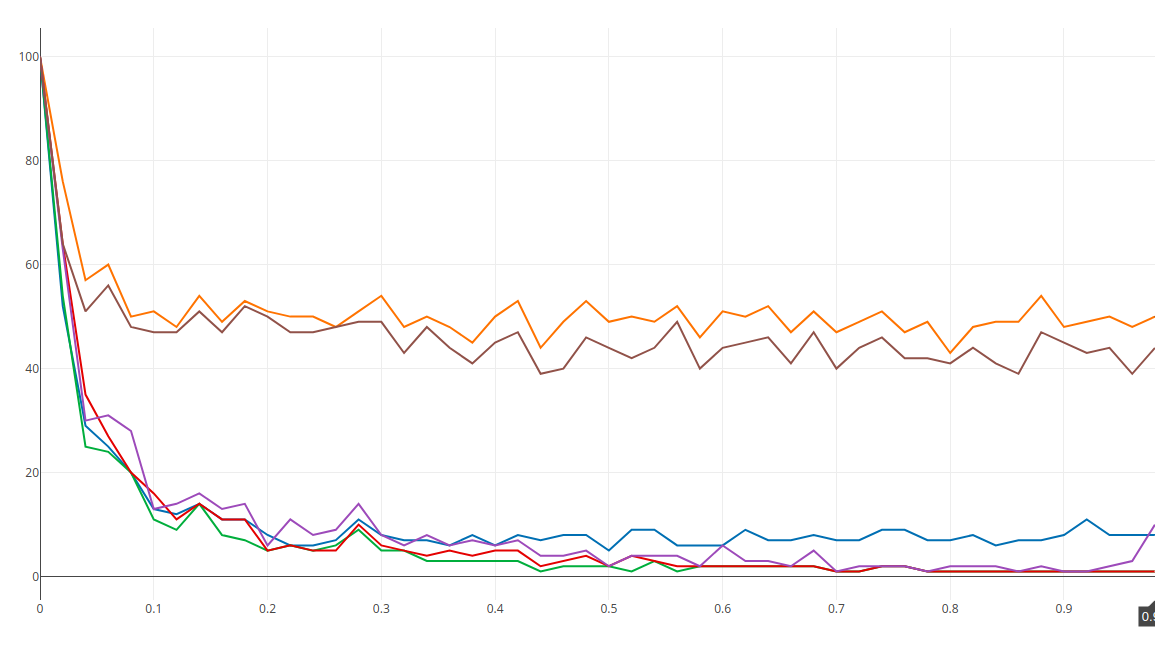
\includegraphics[scale=0.32]{pics/random_count.png}\\
Отношение $c_{dir}/c_{undir}$:\\
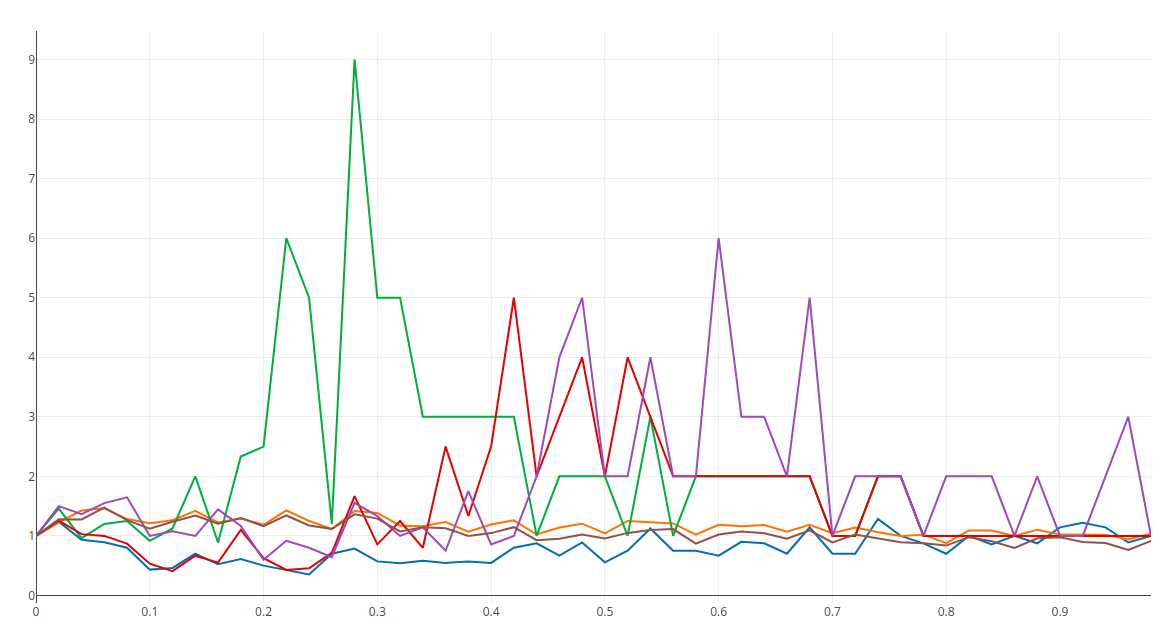
\includegraphics[scale=0.32]{pics/random_d.png}
\newpage
{\bfseries Jaccard distance:} \\
Количество сообществ:\\
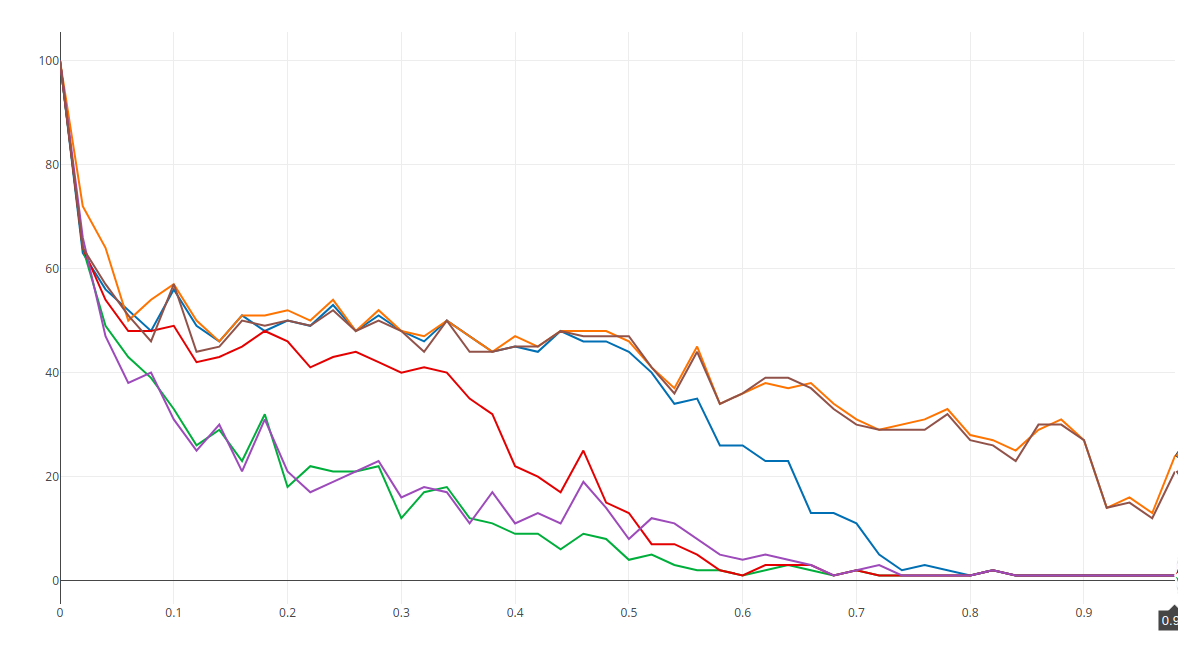
\includegraphics[scale=0.32]{pics/jaccard_count.png}\\
Отношение $c_{dir}/c_{undir}$:\\
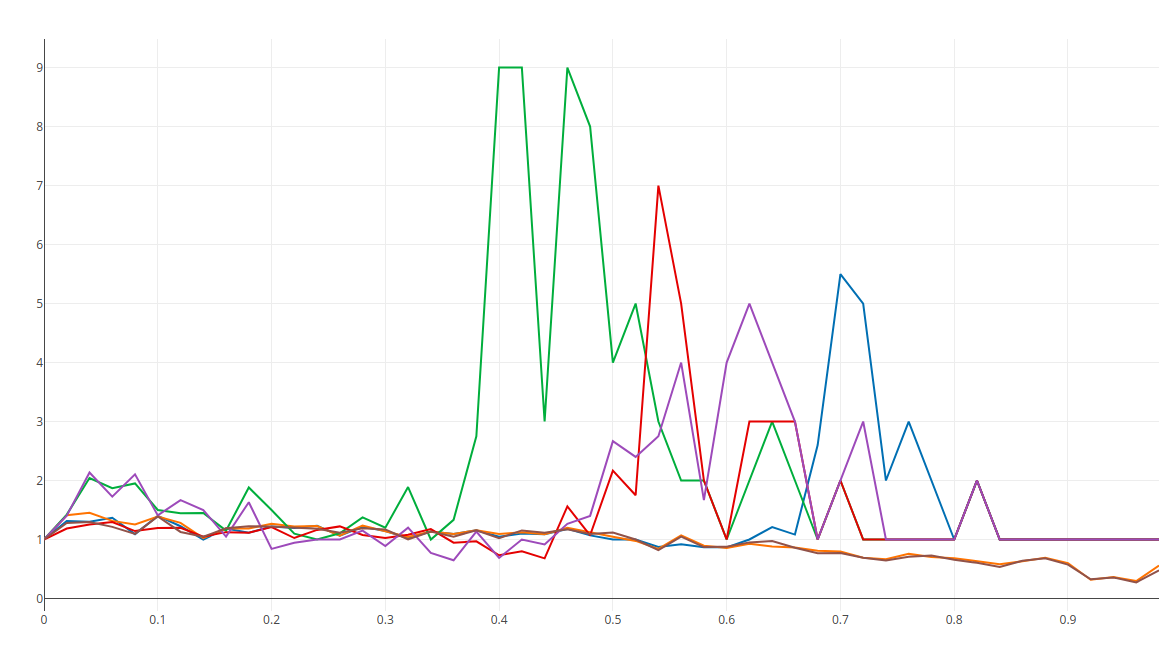
\includegraphics[scale=0.32]{pics/jaccard_d.png}
\newpage
{\bfseries Все веса равны $1/2$:} \\
Количество сообществ:\\
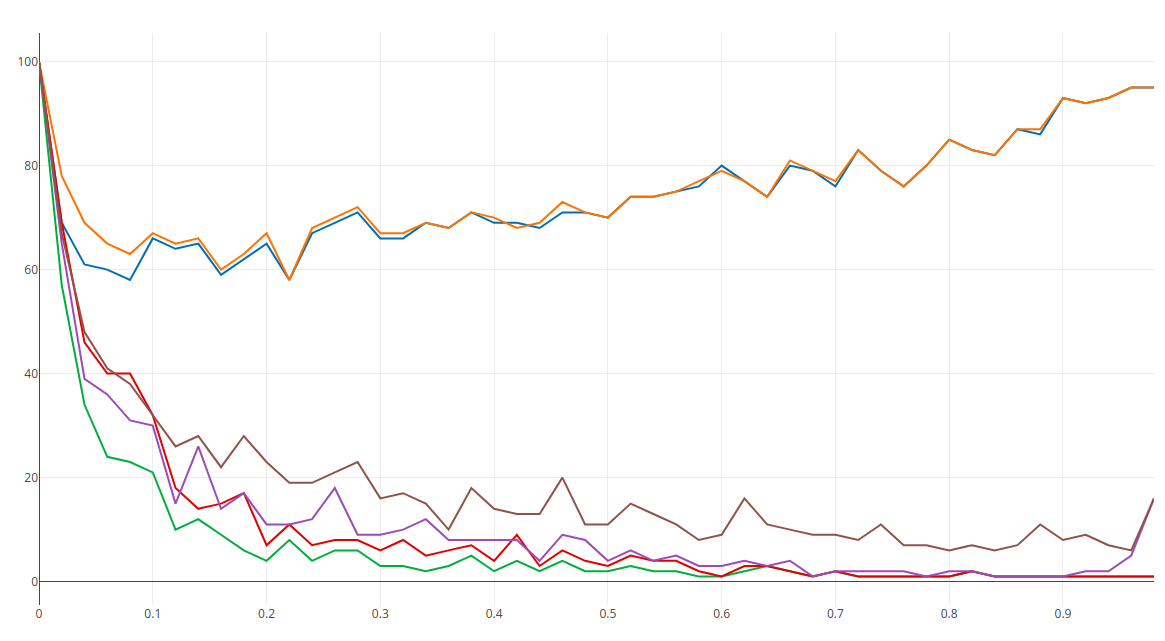
\includegraphics[scale=0.32]{pics/static_count.png}\\
Отношение $c_{dir}/c_{undir}$:\\
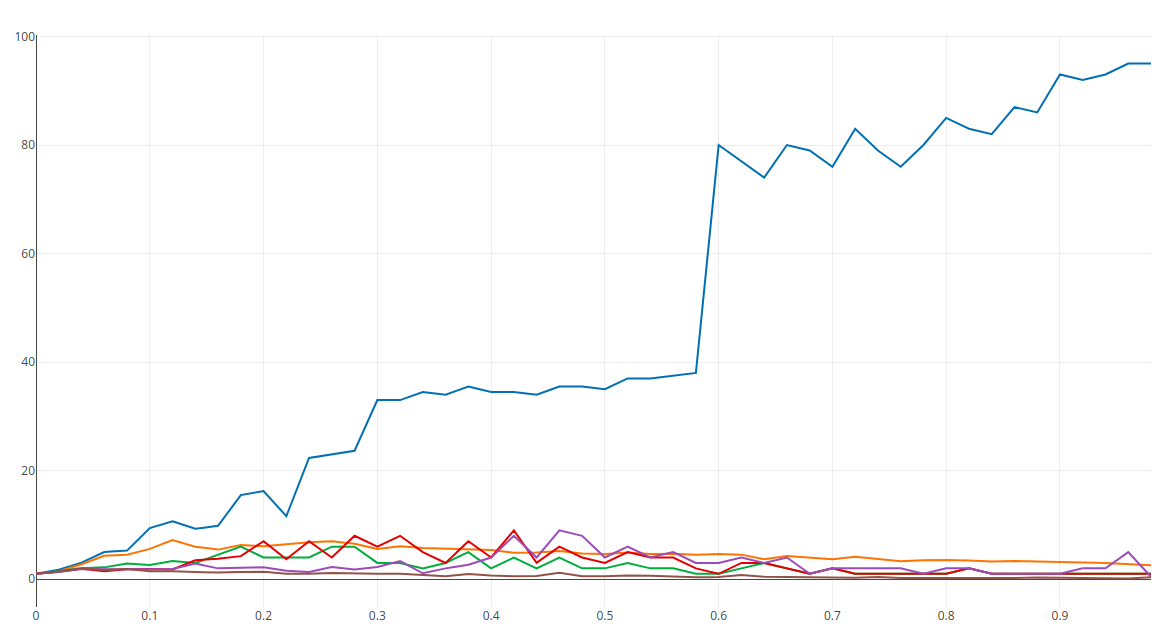
\includegraphics[scale=0.32]{pics/static_d.png}\\